\documentclass[conference]{IEEEtran}
\IEEEoverridecommandlockouts
% The preceding line is only needed to identify funding in the first footnote. If that is unneeded, please comment it out.
\usepackage{cite}
\usepackage{amsmath,amssymb,amsfonts}
\usepackage{algorithmic}
\usepackage{graphicx}
\usepackage{textcomp}
\usepackage{xcolor}
\def\BibTeX{{\rm B\kern-.05em{\sc i\kern-.025em b}\kern-.08em
    T\kern-.1667em\lower.7ex\hbox{E}\kern-.125emX}}
\usepackage{listings}
\lstset{
  frame=single,
  language=python,
  basicstyle=\small,
}

\makeatletter
\def\lst@makecaption{%
  \def\@captype{table}%
  \@makecaption
}
\makeatother

\begin{document}

\title{Benchmarking Agents Across Diverse Tasks}

\author{
\IEEEauthorblockN{Alexander Moore}
\IEEEauthorblockA{\textit{Data Science} \\
\textit{Worcester Polytechnic Institute}\\
Worcester, United States \\
ammoore@wpi.edu}

\and

\IEEEauthorblockN{Brian Lewandowski}
\IEEEauthorblockA{\textit{Computer Science} \\
\textit{Worcester Polytechnic Institute}\\
Worcester, United States \\
balewandowski@wpi.edu}

\and

\IEEEauthorblockN{Jannik Haas}
\IEEEauthorblockA{\textit{Data Science} \\
\textit{Worcester Polytechnic Institute}\\
Worcester, United States \\
jbhaas@wpi.edu}

\and

\IEEEauthorblockN{Quincy Hershey}
\IEEEauthorblockA{\textit{Data Science} \\
\textit{Worcester Polytechnic Institute}\\
Worcester, United States \\
qbhershey@wpi.edu}

\and

\IEEEauthorblockN{Scott Tang}
\IEEEauthorblockA{\textit{Data Science} \\
\textit{Worcester Polytechnic Institute}\\
Worcester, United States \\
stang3@wpi.edu}
}

\maketitle

\begin{abstract}
    Understanding which models succeed and why at which tasks is a foundational experience in reinforcement learning.
    Following a baseline of techniques and best practices found in the literature this project will show a comparison of multiple reinforcement learning techniques applied in a few common environments.
    In particular, this project implements several algorithms under the Q-learning, policy learning, and actor-critic categories and compares the results across several tasks.
    We demonstrate the strengths and weaknesses of a large sample of models on discrete-action and continuous action tasks.
    This work explores a set of baseline results for diverse reinforcement learning algorithms, in order to compare and contrast the performance of models on diverse tasks.
    Results sentence here.
\end{abstract}

\begin{IEEEkeywords}
Q-Learning, Policy Learning, Policy Gradient, Actor-Critic, Reinforcement Learning
\end{IEEEkeywords}

\section{Introduction} \label{intro}
Project 3 explored how to construct a Deep Q Network (DQN) or a similar model by following the classic DQN algorithm outlined originally in \cite{DQNOriginalPaper}.
Building off of this recent experience this project takes the deep learning techniques discussed in class and applies them to several well-known tasks using Q-learning, policy learning, and actor-critic methods. Our group implemented, optimized, and benchmarked a large variety of models from these diverse families in order to analyze and discuss the success and failures of each model. We quantify model success by comparing the scores achieved as well as the time-to-convergence in terms of training episodes needed to reach a threshold score.
The results of these methods are compared and discussed.

The openai gym \footnote{https://gym.openai.com/} was chosen to be used as the game environment.
Two games were chosen to be used for comparison of the algorithms in this paper.
First, the Breakout game was used for its familiarity from Project 3 and that it has a known level of difficulty.
In addition, it serves as a discrete action space environment. The Breakout-v0 game is a productive demonstration as part of the poster presentation since the students in the class are all familiar with the process of implementing, optimizing, and testing a DQN-family model on the game. This will contextualize both the work of the project as well as expected score results, for example 50 for a baseline and 400 for the best-scorers in the course.\footnote{https://github.com/yingxue-zhang/DS595CS525-RL-Projects/tree/master/Project3}
To contrast with this, the MountainCar was also chosen as it has both a discrete and continuous action space environment available for use.
Using these environments multiple agents were implemented, trained, and tested using DQN, Double DQN, Dueling DQN, Multistep DQN, Multistep Double DQN, REINFORCE, Proximal Policy Optimization (PPO), and Advantage Actor Critic (A2C).
A breakdown of where these algorithms are categorized in the field of reinforcement learning can be seen in Figure \ref{fig:agentsImplemented}.

\begin{figure}[htbp]
\centerline{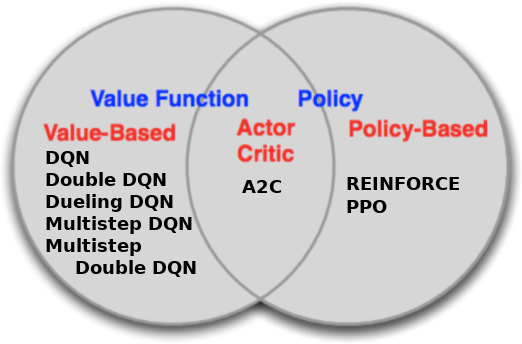
\includegraphics[scale=0.4]{implemented_agents.png}}
\caption{\textbf{Implemented Agents in the field of Reinforcement Learning}  A breakdown of where the implemented agents in this paper are categorized in the wider field of reinforcement learning.}
\label{fig:agentsImplemented}
\end{figure}

This work shows that these algorithms all have strengths and weaknesses in a wide variety of areas including task completion, complexity, training time, and sensitivity to hyperparameters. Ultimately, the success of models is left largely to the hyperparameter selection and tuning steps.

The remainder of this paper is organized as follows:
\begin{itemize}
\item Section \ref{background} provides background information regarding the methods implemented.
\item Section \ref{methodology} provides a description of the methodology used to train, execute, and assess the algorithms explored.
\item Section \ref{results} provides a discussion of the training process and associated results.
\item Finally, the paper concludes in section \ref{conclusion}.
\end{itemize}

\section{Background Information} \label{background}

\subsection{Deep Q Learning}
Deep Q learning uses a deep neural network to learn coefficients $\omega$ such that the network's value function evaluates $(state, action)$ pairs improving the model's task reward. For our Breakout environment this will be a convolution over a stack screen space samples, and for Mountaincar the model is a simple fully-connected network over the state game state: the car position and car velocity.

Deep Q Learning is trained by minimizing the loss taken by evaluating the Q(s,a) value between the agent's state-value function and a target Q function, which is not optimized but occasionally updated to keep the training Q learning.

\subsection{Double Deep Q Learning}
Double deep Q networks address the maximization bias problem from Deep q learning by instead letting two Q functions randomly select the action and update the corresponding Q function. This process inhibits bias and will potentially converge faster or outright outperform DQN on all tasks.

\subsection{Dueling Deep Q Learning}
Dueling DQN separates the Q-learning process into two functions, the sum of the state and state-action estimator models. This approach ideally learns how to relatively value states by accounting for a learned state-value function $V(s)$, as well as an advantage function $A(s,a)$ interpreted as the value of taking action $a$ while in state $s$. For this reason this different approach will be interesting to analyze on tasks where the actions might not always directly affect the environment, for example in breakout where many movements have no direct affect on the game environment.

\subsection{Multistep DQN Models}

\subsection{Basic Policy Gradient}
Policy gradient algorithms in general are methods that learn a parameterized policy that can select actions without consulting a value function \cite{ReinforcementLearningBook}.
A value function may be utilized or learned to support learning a given policy, however, it is not involved in the process of choosing an action with these methods \cite{ReinforcementLearningBook}.
The Basic Policy Gradient algorithm treats learning of the policy as an episodic case using a performance measure that equates to the reward obtained following the current policy given a starting state of an episode. 
At its core, the Basic Policy Gradient algorithm takes the gradient of expected rewards for an episode and uses it to update the policy parameters.
This can be summarized by the two equations below,

$$\nabla \bar{R}_{\theta} = \frac{1}{N} \sum \limits_{n=1}^N \sum \limits_{t=1}^{T_n} R(\tau^n) \nabla log\pi_{\theta}(a_{t}^n | s_{t}^n)$$

$$\theta = \theta  + \eta \nabla \bar{R}_{\theta}$$

where N is the number of episodes, T is the steps within an episode, R is the reward for a given episode, $\theta$ are the policy parameters, a is a given action, and s is a given state.

Implemented in pseudocode, this algorithm would be similar to Listing \ref{listing:basicPolicyGradientAlg}.
While not implemented as part of this project is is the building block for all subsequently developed policy gradient models.

\begin{lstlisting}[
    float=t,
    caption=\textbf{Basic Policy Gradient} The basic policy gradient algorithm,
    label=listing:basicPolicyGradientAlg,
]

Loop until stopping criteria met:
    for a batch of episodes:
        - Step through episode
        - Store reward gained

    - Determine reward gradient of batch
    - Update policy parameters
\end{lstlisting}

\subsection{REINFORCE Policy Gradient}
The REINFORCE Policy Gradient method also referred to as Monte-Carlo Policy Gradient makes a slight adjustment to the Basic Policy Gradient algorithm of using the return from each time step instead of the overall reward from the episode in the update of the policy parameters. This will reduce the high variance of the standard basic policy gradient algorithm.
This change can be seen in the pseudocode in Listing \ref{listing:reinforcePolicyGradientAlg}. 

\begin{lstlisting}[
    float=t,
    mathescape = true,
    caption=\textbf{REINFORCE Policy Gradient} The reinforce policy gradient algorithm,
    label=listing:reinforcePolicyGradientAlg,
]

For each episode from the current policy:
    For t=1 to T-1 do:
        {$\theta = \theta  + \alpha \nabla_{\theta} log\pi_{\theta}(s_t, a_t)G_t$}

    end for
end for
return {$\theta$}
\end{lstlisting}

\subsection{PPO Policy Gradient}
Unlike the Basic and REINFORCE policy gradient algorithms, the Proximal Policy Optimization (PPO) algorithm is an off-policy method, where the performance assessment and improvement of a policy is different than the one used for action selection (or sampling). The separate policies allow the collected data to be used more than once, which result in faster performance. Furthermore, typical policy gradient algorithms perform updates only once per sample while PPO can perform multiple updates with minibatches of each sample. PPO also addresses other shortcomings of the Basic Policy Gradient by subtracting the state-value as the baseline to improve update accuracy when rewards are non-negative via an Advantage function. This function also serves to reduce large variance without increasing bias. Finally, PPO improves stability by imposing a constraint on the distance (or difference) between the old and new policies by clipping their ratio to a small interval around one. Due to this constraint, some critics believe that PPO should be considered an on-policy method.

There are different options for implementing the PPO algorithm, as outlined in \cite{schulman2017proximal}. The one chosen for this work is known as the Actor-Critic Style but with only one actor. The psuedocode is depicted in Listing \ref{listing:PPOPolicyGradientAlg}. The Actor-Critic method, specifically A2C, is described in the next subsection. In addition, entropy bonus and clipping (without the KL divergence penalty) of the surrogate objective function and a decaying learning rate were implemented in this work. Finally, the estimation of advantages followed the Generalized Advantage Estimation (GAE) approach described in \cite{schulman2018highdimensional}.

\begin{lstlisting}[
    float=t,
    mathescape = true,
    caption=\textbf{PPO Policy Gradient, Actor-Critic Style},
    label=listing:PPOPolicyGradientAlg,
]

for $\textnormal{iteration = 1, 2,... do:}$
    for $\textnormal{actor = 1, 2,...,}$ N $\textnormal{do: (N = 1 in this implementation)}$
        $\textnormal{Collect dataset based on policy}$ $\pi_{\theta}_{old}$ $\textnormal{for}$ $\emph{T}$ $\textnormal{steps}$
        $\textnormal{Compute advantages (}$${\hat{A}}_1,..., {\hat{A}}_T$$\textnormal{) using}$
            $\textnormal{Generalized Advantage Estimation (GAE)}$
    $\textnormal{end}$ for
    $\textnormal{Optimize surrogate objective}$ $\emph{L}$ $\textnormal{wrt}$ $\theta$ $\textnormal{by taking}$ $\emph{K}$ $\textnormal{steps}$
        $\textnormal{with minibatch (size}$ $\emph{M} \leq \emph{T}$$\textnormal{) SGD (}$$\emph{Adam}$$\textnormal{)}$
    $\theta_{old} \longleftarrow \theta$
$\textnormal{end}$ for

\end{lstlisting}

\subsection{Advantage Actor Critic}
Actor-Critic methods, similar to the REINFORCE algorithm, learn both a policy function and state-value function.
The main difference between them, however, is the fact that actor-critic methods use the value function as a way to bootstrap the value estimation.
The implementation for this work follows closely to the "One-step Actor-Critic" algorithm outlined in \cite{ReinforcementLearningBook} with some practical updates for implementation and stands as a synchronous adaptation of the Asynchronous Advantage Actor critic algorithm (A3C) presented in \cite{mnih2016asynchronous}.
It is a temporal difference algorithm that relies solely on the current step for learning.
This is in contrast to the many of the other algorithms implemented in this work as they involve utilizing a replay buffer for batch learning.

In addition, it should be noted that this implementation remains a basic implementation and does not include the commonly seen updates added to this method such as an additional entropy loss.

\section{Methodology} \label{methodology}

\subsection{Tools and Framework}
This project used the Python language and several python libraries. 
In addition to the standard libraries, the following additional libraries were used:
 
\begin{itemize}
    \item OpenAI Gym \cite{openaigym}
    \item PyTorch
    \item NumPy
    \item Matplotlib
    \item Pandas
\end{itemize}

The framework provided from Project 3 was built off of and adapted to support additional environments aside from Breakout.
A framework was built such that the main training and testing pipeline was consistent across algorithm implementations.
This allowed for each team member to focus on implementing specific models and algorithm learning details.

The general workflow using this framework can be seen in Listing \ref{listing:basicModelWorkflow}.

\begin{lstlisting}[
    float=t,
    caption=\textbf{Algorithm Development Workflow} The basic workflow used to develop new models and algorithms.,
    label=listing:basicModelWorkflow,
]

# Create a new model in models directory
# - Implement the __init__ function
# - Implement the forward function

# Create a new agent in the agents directory
# - Implement the make_action function
# - Implement the can_train function
# - Implement the train function

# Execute training for model on command line
# python main.py \
#    --train_dqn \
#    --model sample_model.SampleModel \
#    --agent sample_agent.SampleAgent \
#    --other_arguments

\end{lstlisting}

It should be noted that all agents inherit a set of functions from a base class allowing for a small barrier to entry in setting up new agents.
An agent runner class was constructed such that it handles the main training loop used by all algorithms implemented while the learning details are held within the specific agents themselves.

In addition, during model training, this framework stores all arguments used to start the session as well as periodic interim models and statistics in both raw format and as plots.
This allowed for repeatability and easy metrics collection during every session.
An example view of what this archive directory looks like can be seen in Listing \ref{listing:sampleModelArchive}.

\begin{lstlisting}[
    float=t,
    caption=\textbf{Model Training Archive} A typical archive from a model that has been trained for 2000 episodes.,
    label=listing:sampleModelArchive,
]

archive/
   |
   test_learning_rate/
       |
       args.pkl
       1000_model.pth
       1000_optimizer.pth
       1000_training_metrics.csv
       1000_training_reward_plot.png
       1000_test_metrics.csv
       1000_test_reward_plot.png
       2000_model.pth
       2000_optimizer.pth
       2000_training_metrics.csv
       2000_training_reward_plot.png
       2000_test_metrics.csv
       2000_test_reward_plot.png
\end{lstlisting}

\subsection{Gym Environments}
Several different environments from the openai gym python packages were utilized on this project.
A description of each of these environments and a description of the task to be solved by agents within them follows.

\subsubsection{BreakoutNoFrameskip-v4}
The Breakout environment involves interacting with the Atari 2600 game by the agent receiving image data for what has been seen on screen.
After pre-processing handled by the atari wrapper code the state space consists of 4 stacked 84x84 images.
An example of the original environment that would be viewed by a human playing the game can be seen in Figure \ref{fig:atariBreakoutEnvironment}.

\begin{figure}[htbp]
\centerline{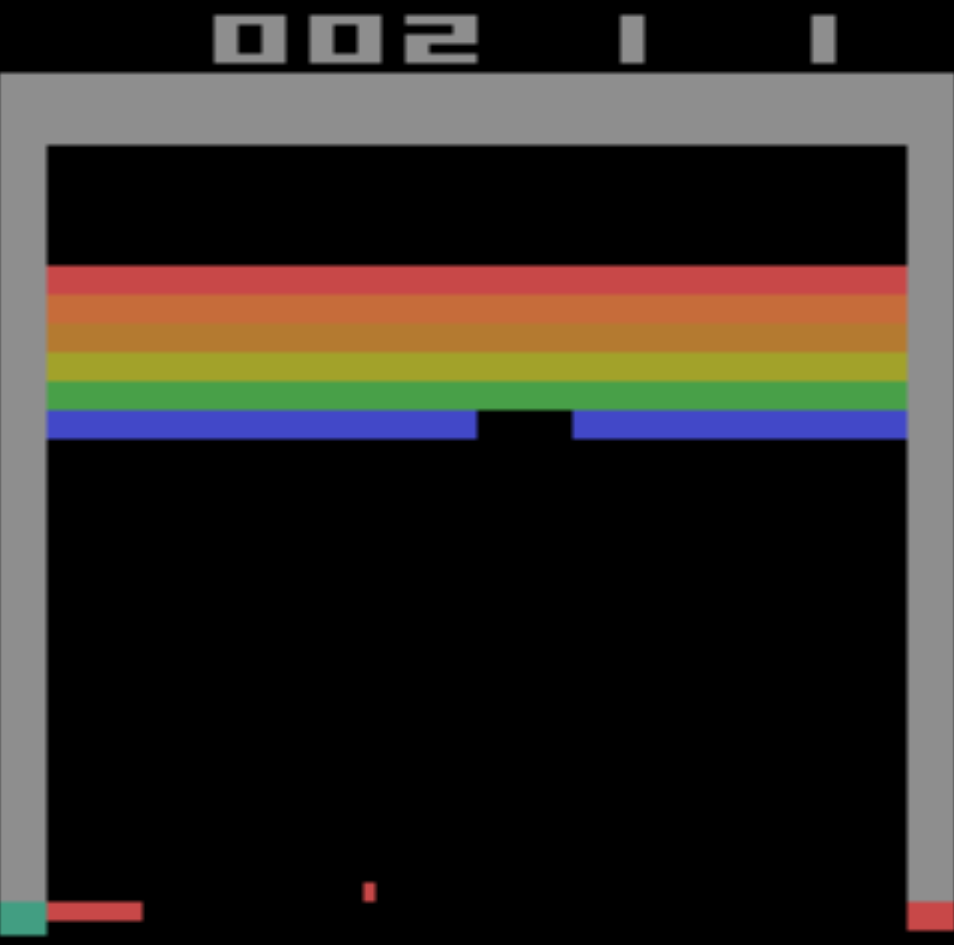
\includegraphics[scale=0.1]{atari_breakout_sample.png}}
\caption{\textbf{Example of the Breakout environment.}  The Atari Breakout environment provided by openai.}
\label{fig:atariBreakoutEnvironment}
\end{figure}

The action space for this environment consists of 4 possible discrete actions:

\begin{itemize}
    \item LEFT - Move agent left
    \item RIGHT - Move agent right
    \item NOOP - Do nothing
    \item FIRE - Places ball in motion at start of new lives
\end{itemize}

This environment was chosen as it was familiar from Project 3 and sufficiently difficult for naive models.
In addition, it serves as a well-contained discrete action space for all algorithms under test.

The reward structure for this environment consists of the traditional values for the blocks in the game where the first two levels provide one point, the next two levels provide 3 points, and the final two levels provide 7 points.
For the learning agent, the atari wrapper environment clips this reward to be just one point for a timestep where a brick was broken.

\subsubsection{MountainCarContinuous-v0}
The Mountain Car environment in both its original and continuous form consists of the agent being a car beginning in the valley between two mountains.
In this classic control task, the agent must apply a specific force to the mountain car with the goal of reaching the top of the right hand mountain as seen by the flag in Figure \ref{fig:mountainCarEnvironment}.

\begin{figure}[htbp]
\centerline{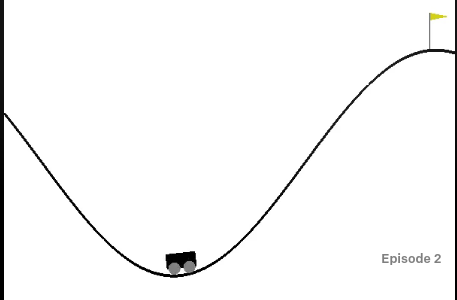
\includegraphics[scale=0.5]{mountain_car.png}}
\caption{\textbf{Example of the Mountain Car Environment}  The mountain car environment provided by openai.}
\label{fig:mountainCarEnvironment}
\end{figure}

In this environment, the agent must learn to gather enough momentum by first going backwards a bit prior to going forwards in order to have enough acceleration to reach the flag.

The state space for this environment consists only of the mountain car's position and velocity.
The action space for this environment is a single continuous action which is the force to be applied to the mountain car.
A positive value is a force towards the goal and a negative value for this force puts the mountain car in reverse.

The reward structure for this environment consists of the agent receiving a small negative reward for the number of actions taken and a positive reward of 100 when reaching the goal.
This environment is considered solved once a score of 90 is achieved \footnote{https://github.com/openai/gym/wiki/MountainCarContinuous-v0}.

This environment was chosen as it is a well-suited introductory environment to explore continuous action spaces.
The game is significantly smaller than the breakout game in terms of state size, as well as being significantly easier to solve, as the optimal strategy is significantly less complex than the space of Breakout strategies.
We expect the training process of this game to be significantly faster than Breakout, letting us train a greater number of agents and optimize the hyperparameters of these agent significantly more than in the Breakout setting.

\subsubsection{MountainCar-v0}
The MountainCar-v0 environment is the discrete action-space relative of MountainCarContinuous-v0 as described above.
This environment entails the same general principles and overall goal but the action space has been altered to use discrete actions as listed below.

\begin{itemize}
    \item PUSH LEFT
    \item PUSH RIGHT
    \item NO PUSH
\end{itemize}

The state-space for this environment remains unchanged.
The reward structure for this environment consists of -1 for each time step until the goal is reached.
The environment is considered solved if an average of -110 points is achieved over 100 consecutive trials \footnote{https://github.com/openai/gym/wiki/MountainCar-v0}.

\subsection{Continuous Action Spaces}
One of the key goals for this project was to interact in an environment with continuous action spaces.
In general, models that operate in discrete action spaces take as input the state space (or state-space and action) and return either a value function or policy function.
The value function represents the value of the particular state and the policy function generally provides an action or probabilities for which actions to execute.

When dealing with continuous action spaces, this is shifted such that the policy learned is the mean and standard deviation for desirable actions within a continuous action space.
As the agent learns, the standard deviation generally starts out wide and then narrows once it is more confident in the actions to take.
Choosing an action consists of sampling from the learned distribution.

\subsection{Continuous Advantage Actor Critic Implementation}
The actor critic implementation follows closely to the "One-step Actor-Critic" algorithm outlined in \cite{ReinforcementLearningBook} with some practical updates made for implementation adapted from Phil Tabor's public codebase \footnote{https://github.com/philtabor}.
This implementation is a temporal difference algorithm using no replay buffer and using only the current time step information to facilitate learning.
In addition, it is implemented in an on-policy manner.

The target for this model was the MountainCarContinuous-v0 environment so the model and agent were structured with this in mind.
One can see the model structure and hyperparameters of the final model in Listing \ref{listing:continuousActorCriticModel} and Table \ref{table:continuousActorCriticHypers} respectively.


\begin{lstlisting}[
  float=t,
  caption=\textbf{Continuous Actor Critic Model}  The model architecture used for the continuous actor critic implementation.,
  label=listing:continuousActorCriticModel,
]
Fully Connected:   2 Input,512 Output
ReLU

|
v

Fully Connected:  512 Input, 512 Output  
ReLU

|\
| \
|  \
|   |
|   v
|  Value Output Layer:  512 Input; 1 Output
|
v

Policy Mean 
Output Layer:   512 Input;  1 Output
tanh

Policy Standard Deviation 
Output Layer:  512 Input;  1 Output
Softplus
\end{lstlisting}

\begin{table}[htbp]
    \caption{\textbf{Continuous Advantage Actor Critic Hyperparameters}  The hyperparameters used for training the continuous actor critic agent.}
\begin{center}
\begin{tabular}{|c|c|c|}
\hline
\textbf{Hyperparameter} & \textbf{Value} \\
\hline
\textbf{Batch Size} & Does not apply \\
\hline
\textbf{Learning Rate} & 0.00015 \\
\hline
\textbf{Replay Buffer Size} & Does not apply \\
\hline
\textbf{Minimum Buffer Training Size} & Does not apply \\
\hline
\textbf{Starting Epsilon} & Does not apply \\
\hline
\textbf{Final Epsilon} & Does not apply \\
\hline
\textbf{Epsilon Decay Steps} & Does not apply \\
\hline
\textbf{Gamma} & 0.99\\
\hline
\textbf{Loss Function} &  -log\_loss * advantage \\
\hline
\textbf{Optimizer} & Adam \\
\hline
\textbf{Target Network Update Interval} & Does not apply \\
\hline
\end{tabular}
\label{table:continuousActorCriticHypers}
\end{center}
\end{table}

\subsection{Continuous PPO Implementation}
As previously stated, our PPO implementation follows the Actor-Critic style. As a result, the structure of the model is identical to that of the one depicted in Listing \ref{listing:continuousActorCriticModel}. Otherwise, the remaining parts of the algorithm are almost identical to the one outlined in the \cite{schulman2017proximal}. Some modifications include the hyperparameter settings and the omission of the KL divergence penalty and a decaying clipping parameter. The hyperparameters for our implementation of the continuous version of the PPO algorithm are shown in Table \ref{table:continuousPPOHypers}.

\begin{table}[htbp]
    \caption{\textbf{Continuous PPO Hyperparameters}  The hyperparameters used for training the continuous PPO agent.}
\begin{center}
\begin{tabular}{|c|c|c|}
\hline
\textbf{Hyperparameter} & \textbf{Value} \\
\hline
\textbf{Steps (T)} & 128 \\
\hline
\textbf{$\#$ of Actors} & 1 \\
\hline
\textbf{Batch Size (M)} & 128 \\
\hline
\textbf{Minibatch Size} & 4 \\
\hline
\textbf{$\#$ of Minibatches} & 32 \\
\hline
\textbf{Network Update Epochs (K)} & 4 \\
\hline
\textbf{Learning Rate} & 0.00015 \\
\hline
\textbf{Learning Rate Decay} & Does not apply \\
\hline
\textbf{Replay Buffer Size} & Does not apply \\
\hline
\textbf{Discount Factor ($\gamma$)} & 0.99 \\
\hline
\textbf{GAE Parameter ($\lambda$)} & 0.95 \\
\hline
\textbf{Prob. Ratio Clipping ($\epsilon$)} & 0.2\\
\hline
\textbf{Clipping Decay} & Does not apply \\
\hline
\textbf{Value Function Loss Coef.} & 0.5 \\
\hline
\textbf{Entropy Coef.} & 0.01 \\
\hline
\textbf{Loss Function} & Surrogate Objective \\
\hline
\textbf{Optimizer} & Adam \\
\hline
\end{tabular}
\label{table:continuousPPOHypers}
\end{center}
\end{table}

\subsection{Discrete Advantage Actor Critic Implementation}
The discrete version of the actor critic algorithm adapted the continuous version discussed earlier for the BreakoutNoFrameskip-v4 environment.
This included incorporating a known model baseline previously shown effective in this environment while adapting it for returning both the policy and values necessary for the actor critic method.

The model structure and hyperparameters for this implementation can be seen in Listing \ref{listing:discreteActorCriticModel} and Table \ref{table:discreteActorCriticHypers} respectively.

\begin{lstlisting}[
  float=t,
  caption=\textbf{Discrete Actor Critic Model}  The model architecture used for the discrete actor critic implementation.,
  label=listing:discreteActorCriticModel,
]
CNN:  32 8x8 filters, stride 4
ReLU

|
v

CNN:  64 4x4 filters, stride 2
ReLU

|
v

CNN:  64 3x3 filters, stride 1
ReLU

|
v

Fully Connected: 3136 Input; 512 Output
ReLU

|\
| \
|  \
|   |
|   v
|  Value Output Layer:  512 Input; 1 Output
|
v

Policy Output Layer: 512 Input;  4 Output
SoftMax
\end{lstlisting}

\begin{table}[htbp]
    \caption{\textbf{Discrete Advantage Actor Critic Hyperparameters}  The hyperparameters used for training the discrete actor critic agent.}
\begin{center}
\begin{tabular}{|c|c|c|}
\hline
\textbf{Hyperparameter} & \textbf{Value} \\
\hline
\textbf{Batch Size} & Does not apply \\
\hline
\textbf{Learning Rate} & 0.0003\\
\hline
\textbf{Replay Buffer Size} & Does not apply \\
\hline
\textbf{Minimum Buffer Training Size} & Does not apply \\
\hline
\textbf{Starting Epsilon} & Does not apply \\
\hline
\textbf{Final Epsilon} & Does not apply \\
\hline
\textbf{Epsilon Decay Steps} & Does not apply \\
\hline
\textbf{Gamma} & 0.99\\
\hline
\textbf{Loss Function} &  -log\_loss * advantage \\
\hline
\textbf{Optimizer} & Adam \\
\hline
\textbf{Target Network Update Interval} & Does not apply \\
\hline
\end{tabular}
\label{table:discreteActorCriticHypers}
\end{center}
\end{table}

\subsection{Discrete PPO Implementation}
The discrete version of the PPO algorithm heavily leveraged the continuous version discussed earlier. The major difference is the incorporation of a convolutional neural network (CNN) based model identical to the one used by the discrete Actor Critic algorithm as depicted in Listing \ref{listing:discreteActorCriticModel}. The hyperparameters for our implementation of the discrete version of the PPO algorithm are shown in Table \ref{table:discretePPOHypers}.

\begin{table}[htbp]
    \caption{\textbf{Discrete PPO Hyperparameters}  The hyperparameters used for training the discrete PPO agent.}
\begin{center}
\begin{tabular}{|c|c|c|}
\hline
\textbf{Hyperparameter} & \textbf{Value} \\
\hline
\textbf{Steps (T)} & 2048 \\
\hline
\textbf{$\#$ of Actors} & 1 \\
\hline
\textbf{Batch Size (M)} & 2048 \\
\hline
\textbf{Minibatch Size} & 4 \\
\hline
\textbf{$\#$ of Minibatches} & 512 \\
\hline
\textbf{Network Update Epochs (K)} & 4 \\
\hline
\textbf{Learning Rate} & 0.0003 \\
\hline
\textbf{Learning Rate Decay} & -2.75e-8 / step \\
\hline
\textbf{Replay Buffer Size} & Does not apply \\
\hline
\textbf{Discount Factor ($\gamma$)} & 0.99 \\
\hline
\textbf{GAE Parameter ($\lambda$)} & 0.95 \\
\hline
\textbf{Prob. Ratio Clipping ($\epsilon$)} & 0.2\\
\hline
\textbf{Clipping Decay} & Does not apply \\
\hline
\textbf{Value Function Loss Coef.} & 0.5 \\
\hline
\textbf{Entropy Coef.} & 0.01 \\
\hline
\textbf{Loss Function} & Surrogate Objective \\
\hline
\textbf{Optimizer} & Adam \\
\hline
\end{tabular}
\label{table:discretePPOHypers}
\end{center}
\end{table}

\section{Results} \label{results}

\subsection{DQN-Family Breakout Results}
With the set of 5 DQN-family models (DQN, Double DQN, Dueling DQN, Multistep DQN, and Multistep DDQN), we did an additional investigation into the importance of the learning rate. For this reason we both benchmark the 5 models with the same low learning rate, then do a comparative experiment of a the same set of models where the only change is a significantly higher learning rate.

\begin{figure}
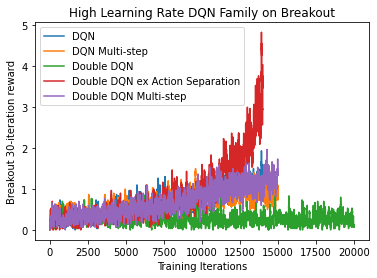
\includegraphics[]{DQNs_breakout_high_train.png}
\caption{The five models show large differences in the ability to quickly improve when using a large learning rate. We see that Double DQN without Action Separation significantly departs from the pack in terms of performance. Though Double DQN fails to learn in 20,000 iterations, the model is implemented correctly, shown by the performance in the low-learning-rate trials.}
\end{figure}


\begin{figure}
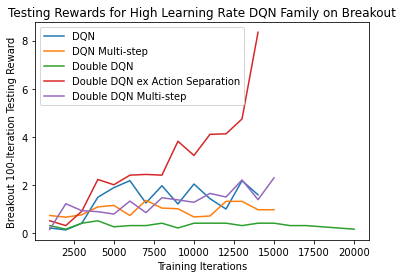
\includegraphics[]{DQNs_breakout_high.png}
\caption{The testing performances shown here and consistent with the training rewards: Double DQN without action seperation drastically outperforms all others in terms of rapid learning acceleration in Breakout.}
\end{figure}

\subsection{DQN-Family MountainCar Results}
For the MountainCar implementation of the DQN family, we expected a larger difference than what we observe here. It is possible that the simple nature of the game in terms of both the state and optimal policy makes it hard for some models to succeed drastically more than others. To a suprising degree, we see the training rewards of all three DQN models highly consistent, both in tertms of the initial acceleration in learning as well as the moment and hieght of the plateau around 1000 iterations to a score around -120.

\begin{figure}
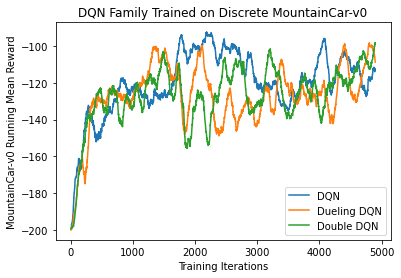
\includegraphics[]{DQN_family_car.png}
\caption{The three DQN models implemented on the discrete MountainCar game show remarkably similar behavior in training.}
\end{figure}

\subsection{Continuous Advantage Actor Critic}
The continuous actor critic agent was exercised using the MountainCarContinuous-v0 environment.
This agent as implemented was able to obtain adequate scores in this game as well as meet the benchmark of 90 that is considered beating the game.
This can be seen in the test reward plot in Figure \ref{fig:actorCriticGoodTestRewardMcc}.
In this plot scores near 80 are achieved for starting at episode 7000 with the highest score coming in at 91.06.

\begin{figure}[htbp]
\centerline{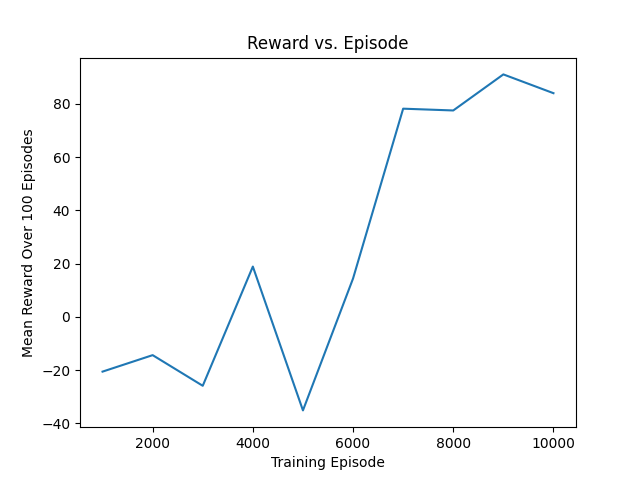
\includegraphics[scale=0.5]{best_actor_critic_mcc_test.png}}
\caption{\textbf{The actor critic agent playing MountainCarContinuous-v0}  The actor critic agent successfully learns how to win the MountainCarContinuous-v0 environment.}
\label{fig:actorCriticGoodTestRewardMcc}
\end{figure}

Figure \ref{fig:fullWinA2CMountainCar} displays the general steps learned by the agent to gain enough momentum to reach the goal.

\begin{figure}[htbp]
\centerline{\includegraphics[scale=0.3]{full_win.png}}
\caption{\textbf{Typical Strategy learned to win Mountain Car.}  The actor critic learned this strategy to win mountain car by rocking  back and forth to gain enough momentum to reach the goal.}
\label{fig:fullWinA2CMountainCar}
\end{figure}

This environment was run multiple times with this same agent to confirm consistency of results.
While this type of result was achieved consistently there were also runs that displayed some of the known issues with the stability of the actor critic method.
Looking at the training plot from a run in Figure \ref{fig:actorCriticBadTrainingMcc},  it can be seen that the agent begins to learn, then ultimately fails to learn after 5000 episodes of training.

This can be compared to the plot of a typical successful training of the agent as seen in Figure \ref{fig:actorCriticGoodTrainingMcc}.
In this plot one can see a pronounced general upward trend in the learning which has essentially converged around 9000 episodes.

\begin{figure}[htbp]
\centerline{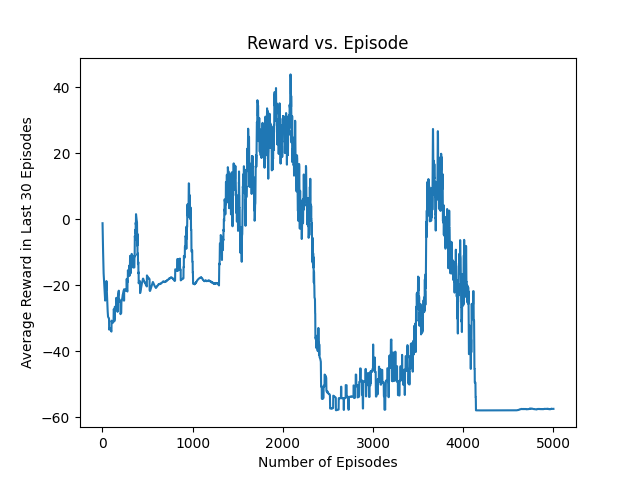
\includegraphics[scale=0.5]{bad_actor_critic_mcc.png}}
\caption{\textbf{A bad training session for actor critic agent playing MountainCarContinuous-v0}  The actor critic method has stability issues that can affect training.}
\label{fig:actorCriticBadTrainingMcc}
\end{figure}

\begin{figure}[htbp]
\centerline{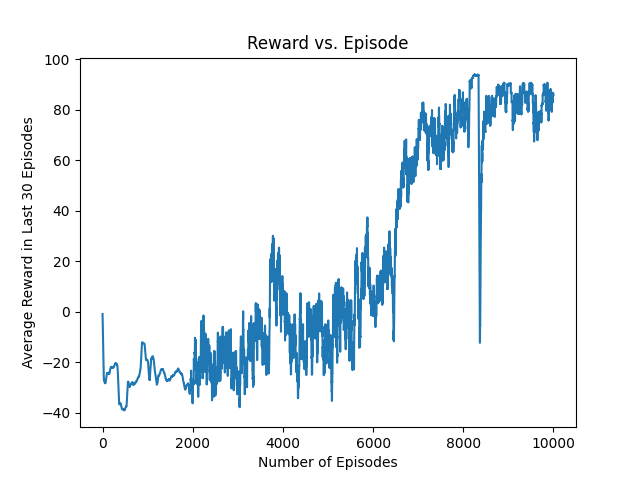
\includegraphics[scale=0.5]{best_actor_critic_mcc.png}}
\caption{\textbf{A typical training session for actor critic agent playing MountainCarContinuous-v0}  A typical training session for the actor critic method.}
\label{fig:actorCriticGoodTrainingMcc}
\end{figure}

\subsection{Discrete Advantage Actor Critic}
The discrete advantage actor critic agent was trained and executed on the BreakoutNoFrameskip-v4 environment.
Through this training we were unable to see significant learning taking place.
The actor critic methods can be sensitive to hyperparameters such as learning rate so a hyperparameter search through multiple learning rates was performed though none of them seemed to affect the learning of the agent.
A summary of these failed attempts can be seen in Figure \ref{fig:actorCriticLearningRateSearch}.

\begin{figure}[htbp]
\centerline{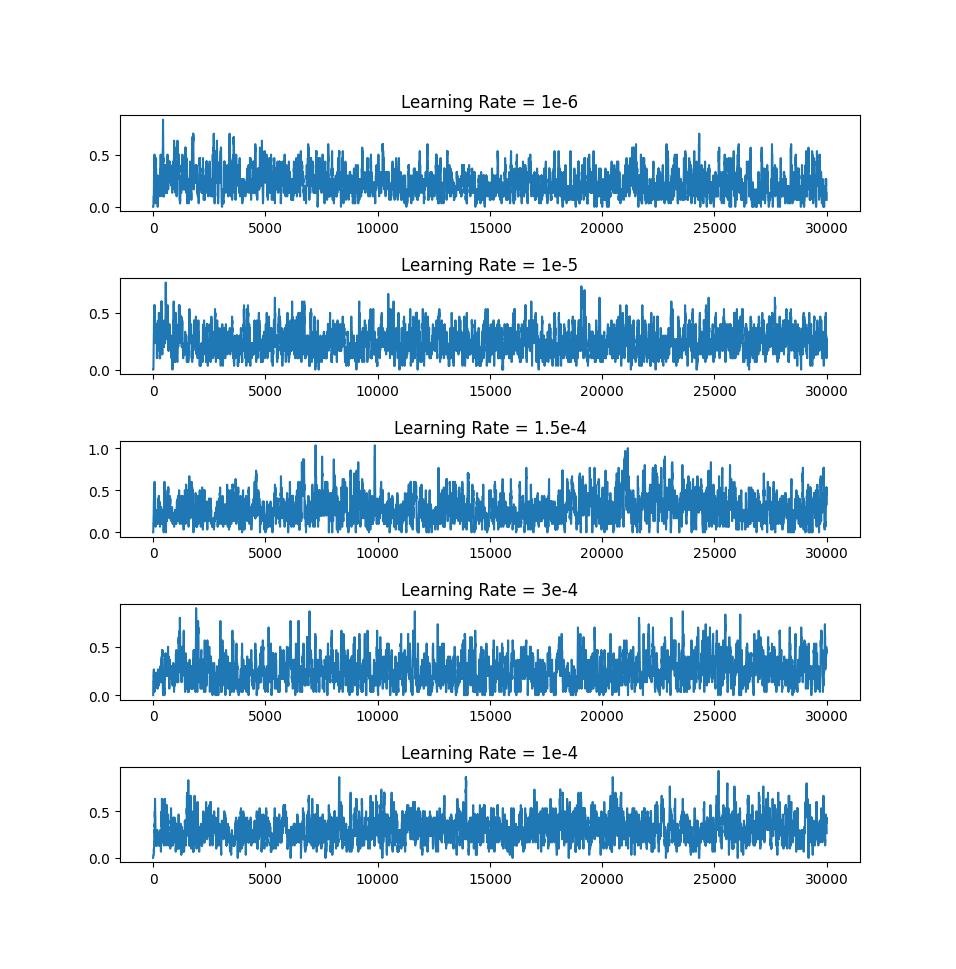
\includegraphics[scale=0.4]{actor_critic_breakout_lr_search.png}}
\caption{\textbf{A search through various learning rates for actor critic on Breakout.}  Changing the hyperparameter for learning rate did not improve the results for the discrete version of actor critic on the Breakout environment.}
\label{fig:actorCriticLearningRateSearch}
\end{figure}

While better results were expected overall for this agent, its implementation lacked essentially all of the hallmark improvements made in \cite{DQNOriginalPaper} and \cite{NatureDeepLearning} such as usage of a target network and replay buffer.
It is suspected that in a future work one may be able to make some of these adjustments such as use of a replay buffer and see improved results.

This result was interesting as it showed an algorithm that performs well in a continuous action space environment did not translate well to one with discrete actions.
One factor affecting this, however, may be the increased complexity of the game of Breakout compared to that of the mountain car problem.

\section{Conclusion} \label{conclusion}
Our discussed findings focus on two primary conclusions: the meta-learning about the process of a research project such as, as well as the findings of results on models.

First, we did get interesting results on the comparison of models on our two tasks. Especially when comparing to Project 3, we find that without exhaustive training and parameter tuning, none of our breakout models were competitive with the kinds of scores found to be possible in the leaderboards. This should contextualize the primary importance of tuning over model selection, and the concession that more complex models do not necessarily outperform simpler models, especially when implementation time, tuning time, and training time are all considered. The training figures demonstrate this complication: though implemented, discrete advantage actor-critic, PPO, and others all failed to get off the ground due to the complications of implementation.

Additionally, the environments selected are as meaningful to the hypothesis as they are hard to select. It is hard to select two or more environments as experimental subjects that can well-discern the differences between models. For example in machine learning, two models can be directly compared over some selection of parameter searching, and quantify their variance and accuracy. However in reinforcement learning, training times for optimization over some set of parameters might be intractable, as well as quantification of their performance can be additionally challenging: are we interested in time-to-convergence? Variability in rewards? Mean reward in testing? These challenges are only exacerbated by the selection of additional games, where the innate complexity of reinforcement learning and the combination of policy, value functions, and agent training all drastically affect the outcome of the model's understanding of the game. For this reason, a few amended research directions are proposed.

As discussed, the scope of models proposed for this project was very wide. A selection of five distinct discrete-action agents as well as four policy gradient agents were all individually implemented from scratch. The additional complication of attempted development over two tasks only complicated this process further. Our goal as discussed in section \ref{intro}, was to compare the performance of models across tasks, with an additional on bench-marking models on each task. The outcome of this ideal proposal would be twofold: a set of results showing with some confidence the relative quality of models on particular results, as well as the pre-trained models which earned those results for future usage. Secondly, this project would show how agents change in *relative* quality as the task changes. Ideally, this comparison could be made over a large set of very diverse tasks: from discrete and continuous actions, large and complex state spaces to very simple ones (such as MountainCar), and strategies of simple and complex nature. This could be a fascinating results to have even an approximation of, which would serve both novice reinforcement learning students with an brief understanding of what works and why, as well as for experts seeking a benchmark for agents which generally thrive at certain tasks, such as learning simple strategies very quickly.

\bibliography{citations.bib}{}
\bibliographystyle{plain}

\vspace{12pt}

\end{document}
